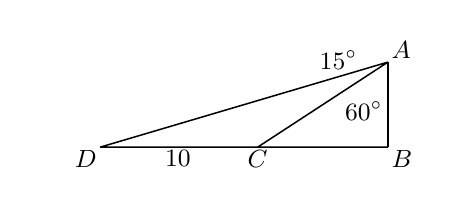
\begin{tikzpicture}[x=.023cm,y=-.023cm,baseline=(current bounding box.center),line width=.55pt,
  every node/.style={font=\small,inner sep=1pt}]
  \path[use as bounding box] (0,0) rectangle (223,85);
  \coordinate (D) at (40,66);
  \coordinate (C) at (127,66);
  \coordinate (B) at (199,66);
  \coordinate (A) at (199,19);
  \draw (D)--(B) (D)--(A) (C)--(A) (B)--(A);
  \node[below left] at (D) {$D$};
  \node[below] at (C) {$C$};
  \node[below right] at (B) {$B$};
  \node[above right] at (A) {$A$};
  \node[below] at (83,66) {$10$};
  \node[above left] at (184,25) {$15^\circ$};
  \node[below left] at (198,39) {$60^\circ$};
\end{tikzpicture}
